\documentclass[border=10pt]{standalone}

\usepackage{tikz}
\usepackage{tikzsymbols}
\usetikzlibrary{calc,patterns,shapes.geometric}

\def\centerarc[#1](#2)(#3:#4:#5){\draw[#1] ($(#2)+({#5*cos(#3)},{#5*sin(#3)})$) arc (#3:#4:#5);}

\begin{document}
	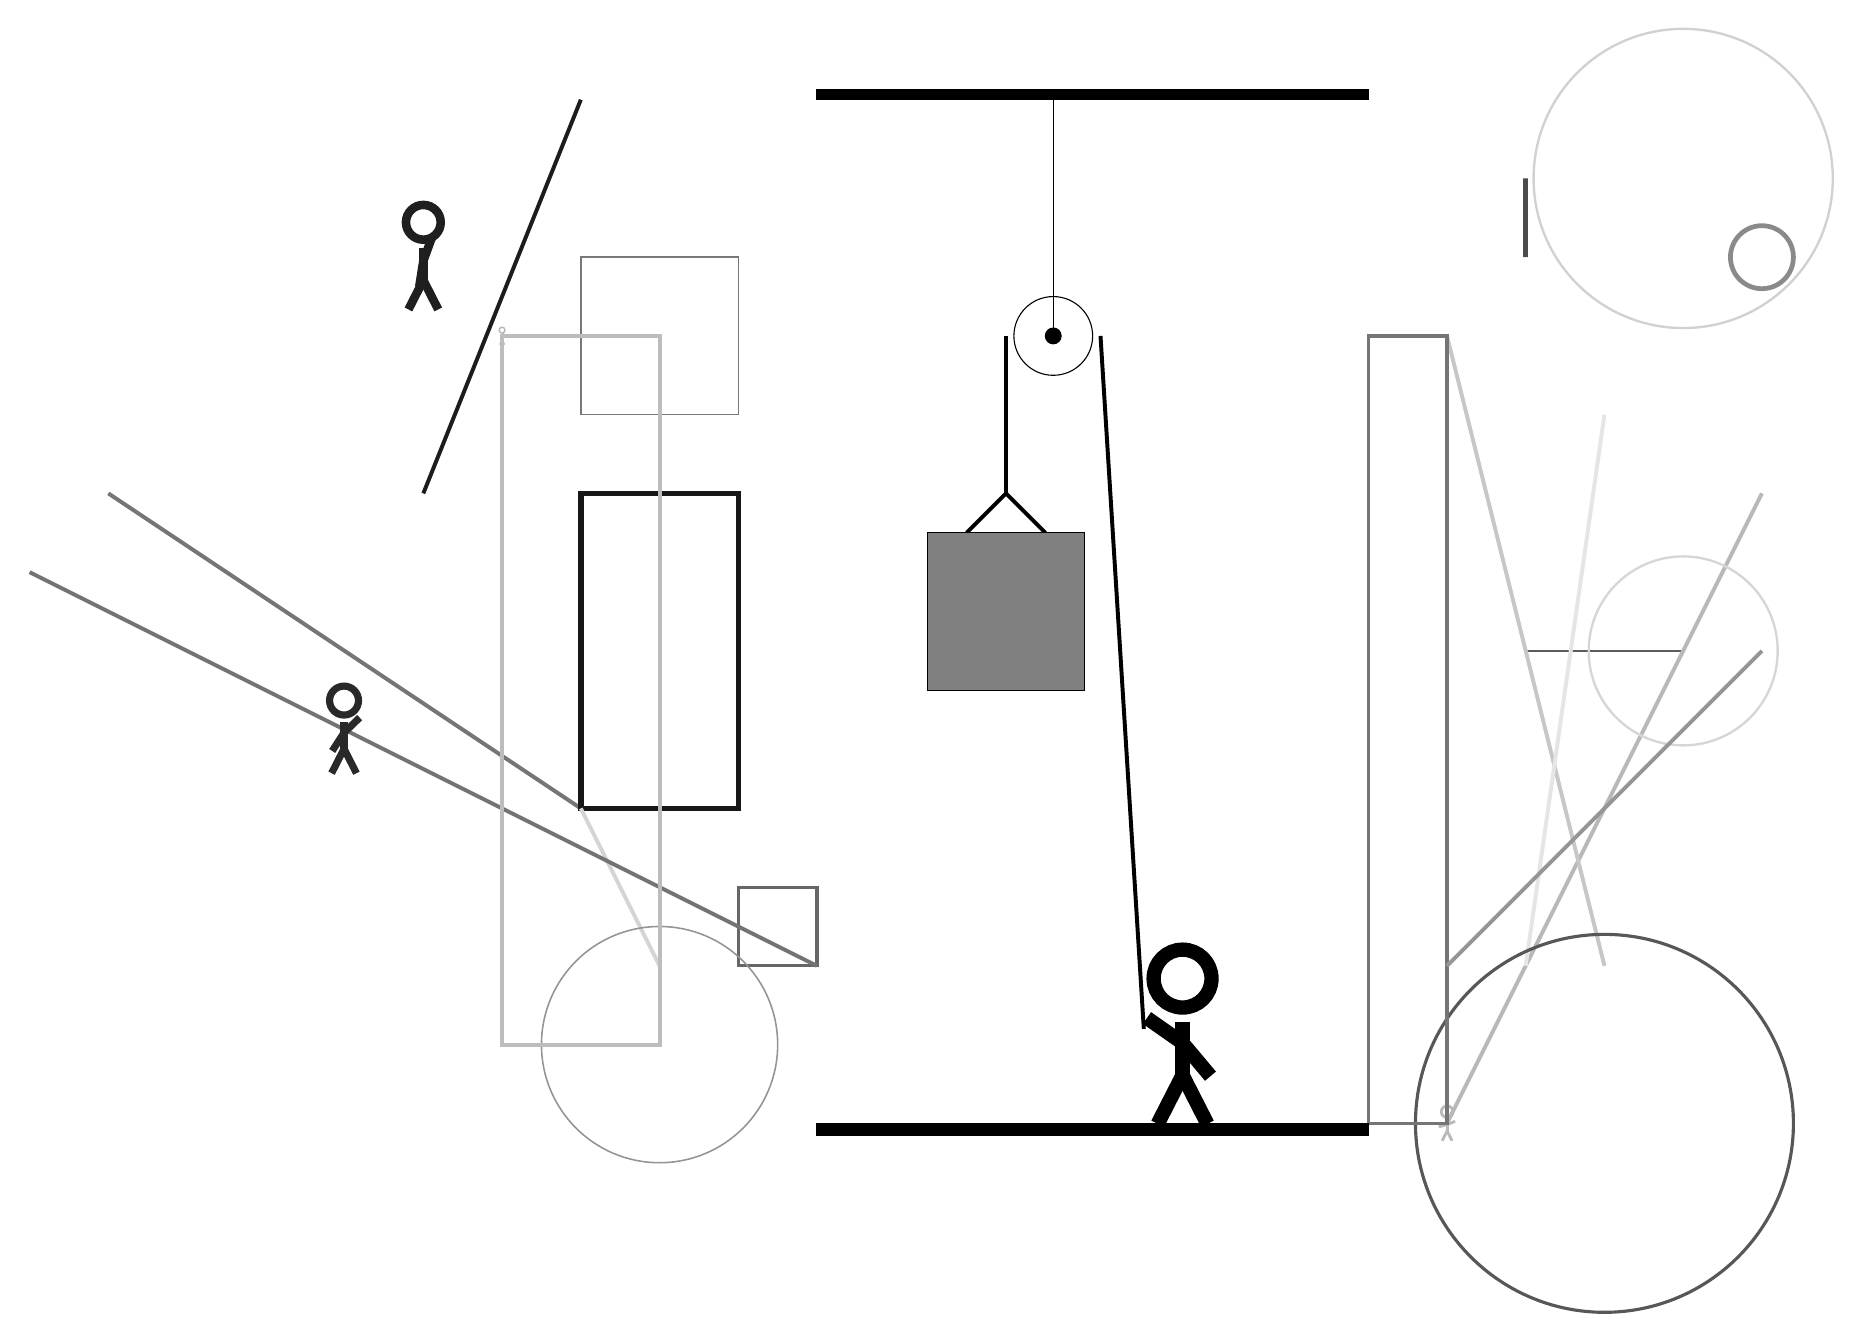
\begin{tikzpicture}
		%%%%% START %%%%%
		
		\draw[fill=black] (-2, 10) rectangle (5, 10.125);
		
		\draw (1, 7) circle (0.5);
		\draw[fill=black] (1, 7) circle (0.1);
		\draw (1, 10) -- (1, 7);
		
		\draw[line width=0.5mm] (-0.1, 4.5) -- (0.4, 5.0) -- (0.9, 4.5);
		\draw[fill=black!50] (-0.6, 4.5) rectangle (1.4, 2.5);
		
		\draw[line width=0.5mm] (0.4, 7) -- (0.4, 5.0);
		\centerarc[line width=0.5mm](1, 7)(0:180:0.6);
		\draw[line width=0.5mm](1.6, 7) -- (2.15, -1.8);
		
		\draw[line width=0.5mm, color=black!80](-5, 4) -- (-5, 4);
		
		\draw[line width=0.2mm, color=black!35] (6, -2) rectangle (6, 2);
		\node[line width=0.3mm, color=black!27] at (6, -3) {\Strichmaxerl[2][15][22]};
		\draw[line width=0.2mm, color=black!64] (7, 3) rectangle (9, 3);
		
		\draw[line width=0.5mm, color=black!54](-5, 1) -- (-11, 5);
		\draw [line width=0.6mm, color=black!46](10, 8) circle (0.4);
		\draw[line width=0.5mm, color=black!28](6, -3) -- (10, 5);
		\draw[line width=0.7mm, color=black!91] (-3, 1) rectangle (-5, 5);
		\draw[line width=0.4mm, color=black!60] (-3, 0) rectangle (-2, -1);
		\draw[line width=0.7mm, color=black!70] (7, 8) rectangle (7, 9);
		\draw [line width=0.3mm, color=black!18](9, 9) circle (1.9);
		
		\draw [line width=0.2mm, color=black!51](11, 1) circle (0.0);
		\node[line width=0.6mm, color=black!88] at (-7, 8) {\Strichmaxerl[6][81][70]};
		
		\draw[line width=0.5mm, color=black!22](8, -1) -- (6, 7);
		\draw[line width=0.5mm, color=black!17](-5, 1) -- (-4, -1);
		\draw [line width=0.2mm, color=black!42](-4, -2) circle (1.5);
		
		\draw [line width=0.3mm, color=black!16](9, 3) circle (1.2);
		
		\draw[line width=0.5mm, color=black!10](7, -1) -- (8, 6);
		\draw [line width=0.4mm, color=black!66](8, -3) circle (2.4);
		\draw[line width=0.5mm, color=black!89](-5, 10) -- (-7, 5);
		\node[line width=0.6mm, color=black!28] at (-6, 7) {\Strichmaxerl[1][80][71]};
		\draw[line width=0.5mm, color=black!55](-2, -1) -- (-12, 4);
		
		\draw[line width=0.4mm, color=black!54] (5, 7) rectangle (6, -3);
		\draw[line width=0.2mm, color=black!53] (-3, 6) rectangle (-5, 8);
		\draw[line width=0.5mm, color=black!26] (-4, -2) rectangle (-6, 7);
		
		\draw[line width=0.5mm, color=black!41](10, 3) -- (6, -1);
		
		\node[line width=0.5mm, color=black!84] at (-8, 2) {\Strichmaxerl[5][57][44]};
		
		\node at (2.6, -1.9) {\Strichmaxerl[10][-35][-50]};
		
		\draw[fill=black] (-2, -3) rectangle (5, -3.15);
		
		%%%%% END %%%%%
	\end{tikzpicture}
\end{document}